%%%%%%%%%%%%%%%%%%%%%%%%%%%%%%%%%%%%%
% Read the /ReadMeFirst/ReadMeFirst.tex for an introduction. Check out the accompanying book "Better Books with LaTeX" for a discussion of the template and step-by-step instructions. The template was originally created by Clemens Lode, LODE Publishing (www.lode.de), mail@lode.de, 8/17/2018. Feel free to use this template for your book project!
%%%%%%%%%%%%%%%%%%%%%%%%%%%%%%%%%%%%%

% Selecting document class scrbook to be in the two-page mode and accommodate for the binding of a printed book.
% The bibliography receives an entry in the table of contents but no number.
\documentclass[pagesize=auto,bibliography=totocnumbered]{scrbook}
\title{Clemens Lode's LaTeX Book Template}
\usepackage{titlesec}
\usepackage{listings}
\titleformat{\section}
{\color{red}\normalfont\Large\bfseries}
{\color{red}\thesection}{1em}{}
% activate babelEN
\usepackage[american]{babel}
% activate babelDE
%\usepackage[ngerman]{babel}


% add a list of words to enforce a certain hyphenation for them.
%\usepackage[T1]{fontenc}
% \usepackage{xspace}
% \usepackage{hyphenat}
% \hyphenation{}

% load additional LaTeX libraries.
% Activate warnings about outdated / invalid packages
%\RequirePackage[l2tabu, orthodox]{nag}

% Provide full error messages
\errorcontextlines 10000

% Enables checking if XeLaTeX is used.
\usepackage{ifxetex}

% Load additional packages for the PDF output
\ifxetex
	% adjusting figures to fit into the width of a page.
	\usepackage{adjustbox}
    
	% Fancy lines for chapters and end of sections.
	\usepackage{psvectorian}
\else
	% Ignore adjustbox commands (HTML files do not have a width).
	\newcommand{\adjustbox}[2][]{#1}

	% Ignore psvectorian lines.
	\newcommand{\psvectorian}[2][]{}

\fi

% Translate horizontal rule and emdash into hrule / "---"
\ifx\HCode\undefined 
	\def\myrule{\hrule}
	\newcommand{\emdash}[1][]{\hspace{0pt}---\hspace{0pt}}
	\newcommand\nextpage[1][]{\newpage}      
\else
	\def\myrule{\HCode{<hr style="clear: both" />}}
	\def\emdash{\HCode{&\#8212;}}
    \newcommand\nextpage[1][]{\HCode{<mbp:pagebreak />}}
\fi


% load our own packages
% Fix PDF creation
\ifxetex
	\let\pdfstrcmp\strcmp
\fi

% this is the macro to define phrases in two languages:
\newcommand{\babelDE}[1]{\ifnum\pdfstrcmp{\languagename}{ngerman}=0 {#1}\fi}
\newcommand{\babelEN}[1]{\ifnum\pdfstrcmp{\languagename}{american}=0 {#1}\fi}

% allow hyphenation recommendation for LaTeX with "=
\useshorthands{"}
\addto\extrasenglish{\languageshorthands{ngerman}}

% Rename the table of contents depending on the used language.
\babelDE{\renewcommand{\contentsname}{Inhaltsverzeichnis}}
\babelEN{\renewcommand{\contentsname}{Table of Contents}}


% Set up bibliography.

% Advanced handling of quotation marks -> important for bibliography.
\usepackage{csquotes}

\ifxetex
% See https://www.ctan.org/pkg/biblatex for documentation.
	\usepackage[indexing=cite,style=authortitle,sortlocale=de_DE,natbib=true]{biblatex}
	\babelDE{\addbibresource{bibliography/german.bib}}
	\babelEN{\addbibresource{bibliography/english.bib}}
\else
	\usepackage{natbib}
	\usepackage{usebib}
	\babelDE{\bibinput{bibliography/german}}
	\babelEN{\bibinput{bibliography/english}}

	% \citetitle does not work with natbib / pdfLaTeX -> translate into \usebibentry
	\newcommand{\citetitle}[2][]{\textit{\usebibentry{#2}{title}}}
\fi

% Set bibliography to footnote size
\renewcommand{\bibfont}{\footnotesize}

\newcommand{\bibpreface}[1]{\patchcmd{\thebibliography}{\list}{#1\list}{}{}}

% Write the name of a referenced section or chapter label with \nameref{label}.
\usepackage{nameref}
% Select a book format

%\usepackage[paperwidth=12.5cm,  paperheight=19.0cm, inner=0.80in, outer=0.3in, top=0.7in, bottom=0.5in]{geometry}
%\usepackage[paperwidth=13.0cm,  paperheight=19.0cm, inner=0.80in, outer=0.3in, top=0.7in, bottom=0.5in]{geometry}
%\usepackage[paperwidth=12.85cm, paperheight=19.84cm, inner=0.80in, outer=0.3in, top=0.7in, bottom=0.5in]{geometry}
%\usepackage[paperwidth=5in,  paperheight=8in, inner=0.80in, outer=0.3in, top=0.7in, bottom=0.5in]{geometry}
\usepackage[paperwidth=5.25in,  paperheight=8in, inner=0.80in, outer=0.3in, top=0.7in, bottom=0.5in]{geometry}
%\usepackage[paperwidth=13.34cm, paperheight=20.32cm, inner=0.80in, outer=0.3in, top=0.7in, bottom=0.5in]{geometry}
%\usepackage[paperwidth=14.8cm,  paperheight=21.0cm, inner=0.80in, outer=0.3in, top=0.7in, bottom=0.5in]{geometry} % DinA5
%\usepackage[paperwidth=13.5cm,  paperheight=21.5cm, inner=0.80in, outer=0.3in, top=0.7in, bottom=0.5in]{geometry}
%\usepackage[paperwidth=13.97cm, paperheight=21.59cm, inner=0.80in, outer=0.3in, top=0.7in, bottom=0.5in]{geometry}
%\usepackage[paperwidth=15.24cm, paperheight=22.86cm, inner=0.80in, outer=0.3in, top=0.7in, bottom=0.5in]{geometry}
%\usepackage[paperwidth=15.6cm,  paperheight=23.39cm, inner=0.80in, outer=0.3in, top=0.7in, bottom=0.5in]{geometry}
%\usepackage[paperwidth=19.05cm, paperheight=23.5cm, inner=0.80in, outer=0.3in, top=0.7in, bottom=0.5in]{geometry}
%\usepackage[paperwidth=16.99cm, paperheight=24.41cm, inner=0.80in, outer=0.3in, top=0.7in, bottom=0.5in]{geometry}
%\usepackage[paperwidth=18.9cm,  paperheight=24.61cm, inner=0.80in, outer=0.3in, top=0.7in, bottom=0.5in]{geometry}
%\usepackage[paperwidth=17.78cm, paperheight=25.4cm, inner=0.80in, outer=0.3in, top=0.7in, bottom=0.5in]{geometry}
%\usepackage[paperwidth=20.32cm, paperheight=25.4cm, inner=0.80in, outer=0.3in, top=0.7in, bottom=0.5in]{geometry}
%\usepackage[paperwidth=21.59cm, paperheight=27.94cm, inner=0.80in, outer=0.3in, top=0.7in, bottom=0.5in]{geometry}




% Sets the font specifications for the chapter lead-in and title.
\newcommand{\chapterLeadinFont}{\Large}
\newcommand{\chapterTitleFont}{\Huge \MakeUppercase }
%
% Lengths used in the chapter title page setup. You can change the values I gave these using the "setlength" commands immediately following the length definitions. Most of these interact with each other. For example, increasing one of the gaps between the bounding rectangles decreases the maximum title width.
%
% The next three lengths adjust the size of the bounding rectangles on chapter title pages by decreasing the lengths of their sides. Increasing these lengths make the rectangles smaller. These rectangles are always centered in the text area so they should adjust to changes in your margins and paper size. The default, outer rectangle (0pt) lies on the margin. All of these lengths should be greater than or equal to zero.
\newlength{\outerRec}\setlength{\outerRec}{0pt}
\newlength{\middleRec}\setlength{\middleRec}{2pt}
\newlength{\innerRec}\setlength{\innerRec}{12pt}
%
% The next three lengths set the edge widths of the rectangles. I did not think these and the previous lengths should interact, so, if you increase these, you may need to adjust the above; otherwise, the edges of two adjacent rectangles may overlap.
\newlength{\outerLineWidth}\setlength{\outerLineWidth}{.5pt}
\newlength{\middleLineWidth}\setlength{\middleLineWidth}{.5pt}
\newlength{\innerLineWidth}\setlength{\innerLineWidth}{.5pt}
%
% Remark: You can comment one of the \draw commands in the code that follows if you want two rectangles. You can also give middle and inner lengths above the same values. 
%
% The next length sets both the left and right distances between the inside of the edge of the inner rectangle and the maximum chapter title width. A positive value ensures that the chapter title lies inside the inner rectangle. If you set this length to 0pt, a longer chapter title may touch the left and right edges of the inner rectangle.
\newlength{\adjustTitleWidth}\setlength{\adjustTitleWidth}{.8cm}
%
% The next lengths, used in the \titlespacing command, set horizontal and vertical title information distances.
\newlength{\leftMar}\setlength{\leftMar}{0pt}% Increases the left margin of the title. Normally, you should not adjust this length.
\newlength{\beforeSep}{\setlength{\beforeSep}{45pt}}% Sets the vertical between the top margin, not the inner rectangle, and the chapter lead-in.
\newlength{\spaceToRule}\setlength{\spaceToRule}{.45cm}% Set vertical spacing between chapter lead-in and the rule. 
\newlength{\spaceAfterRule}{\setlength{\spaceAfterRule}{.75cm}}% Sets the vertical spacing between the rule and the chapter title.
%
% The next length deals with the special chapter titles "Contents" and "Bibliography". It increases the distance between the upper edge of the inner rectangle and the title text.
\newlength{\specialMargin}\setlength{\specialMargin}{3.4cm}
%
\newlength{\topSep}\setlength{\topSep}{0cm}% Sets the vertical space between the top margin and the first line of text on the first text page of a chapter.
%
% The next length compensates for the binding margin. Normally, you should not change this value regardless of your binding margin value.
%\newlength{\adjustForBindingMargin} %
%    \setlength{\adjustForBindingMargin}
%    {\oddsidemargin/2-\evensidemargin/2}
%%%%%
% script to create a full page for the chapter showing the chapter title. The second parameter is the label.
\usepackage{titlesec}
\usepackage{scrhack}

\newenvironment{chapterpage}[3][]{
	\renewcommand*{\chapterpagestyle}{empty}
	\begingroup
	\chapterbox

	\chapter{#2}\label{#3}

	\begin{center}
		\psvectorian[height=10mm]{75}
	\end{center}

    \ifxetex
	    \vspace*{\fill}
	\fi
	\begin{center}

		\ifxetex
			\begin{minipage}{.85\textwidth}
		\fi

		#1
}
{

		\vspace*{15mm}
		\ifxetex
			\end{minipage}
		\fi
	\end{center}

	\endgroup
	\ifxetex
	    \blankpage
	\fi
	\renewcommand*{\chapterpagestyle}{plain}
	\pagestyle{scrheadings}

}

% A script to finalize the page and add an empty page.
\usepackage{afterpage}
\newcommand{\blankpage}{\afterpage{\null\thispagestyle{empty}\nextpage}{\pagestyle{empty}\cleardoublepage}}

% Header and footer configuration
\usepackage[automark,headsepline]{scrpage2}
\pagestyle{scrheadings}

% inner and outer head (relating to pages of a book): put chapter/section title in the middle and the page numbers on the sides.
\ihead[\headmark]{\headmark}\ohead{\pagemark}

% alternating chapter / section titles at the top of the page
\automark[section]{chapter}

% Make heading of each page italics and small capitals.
\renewcommand*{\headfont}{\itshape\scshape}

% Name of the chapter (\chapapp), number of the chapter (\thechapter) and no period (\autodot)
\renewcommand*{\chaptermarkformat}{\chapapp~\thechapter\autodot\enskip}

% prevent splitting footnotes over several pages, see https://texfaq.org/FAQ-splitfoot
\interfootnotelinepenalty=10000

% Set line separator between items in an itemize environment to 5pt 
\usepackage{enumitem}
\setlist[itemize]{parsep=5pt}

% Set the space between paragraphs and deactivate indentation for paragraphs
\setlength{\parskip}{1.4\baselineskip}
\setlength{\parindent}{0pt}

% Set font size of captions to small, the font size of index to very small, and the footnote font size to very small.
%\usepackage[labelfont=bf]{caption}
%\captionsetup{font=small}
\usepackage{imakeidx}
\indexsetup{othercode=\footnotesize}
\renewcommand{\footnotesize}{\scriptsize}

% you can use ``same'' (same font as your document's), ``sf'', ``tt''  or ``rm'' for monospaced font, also see https://www.ctan.org/pkg/url
\usepackage{url}
\urlstyle{same}

% Font tweaks not available for e-books.
\ifxetex

% Slightly tweak font spacing for aesthetics.
	\usepackage{microtype}
	\usepackage{lmodern}

% Use Linux Libertine font. For other fonts, check out http://www.tug.dk/FontCatalogue/
	\usepackage{libertine}
\else
\fi


% prefer more spaces between words rather than more hyphenations at the end of a line
\sloppy
% Tikz configuration. For details, see the main manual at  http://www.texample.net/media/pgf/builds/pgfmanualCVS2012-11-04.pdf
\usepackage{tikz}
\usepackage{tikzpagenodes}
\usepackage{nameref}
\usepackage{booktabs}
\usepackage{csquotes}
\usepackage{siunitx}
\DeclareSIUnit{\sr}{sr}
\usepackage{pgfplots}
% Add support to force LaTeX to put figures at a certain place.
\usepackage{float}

% Set the version for tikz. You can change it to "newest" to always have the current version. The advantage of setting it to a specific version is that your images are always generated the same way, even if the tikz installation is updated. Set it to a newer version if you need functionality (or bugfixes) from that newer version. Also see https://tex.stackexchange.com/questions/139690/dos-and-donts-of-pgfplotssetcompat-newest
\pgfplotsset{compat=1.14}

% Load various tikz libraries, you might need only some of them (or additional ones).
\usetikzlibrary{matrix,calc,positioning,shapes.arrows,shapes.symbols,decorations.pathreplacing,patterns,shapes,backgrounds,lindenmayersystems,shadings,intersections}

% Define styles of various tikz elements.
\tikzstyle{every node}=[font=\small,node distance=40pt and 50pt,thick]
\tikzstyle{textbox} = [rounded corners, text width=60pt, minimum height=50pt,text centered,draw=black]
\tikzstyle{arrow} = [thick,->,>=latex]
\tikzstyle{largearrow} = [thick,right of=book,draw,single arrow head indent=0ex,single arrow, rotate=90,node distance=130pt,text width=160pt,text centered]
\tikzstyle{block} = [rectangle,textbox]
\tikzstyle{textarr} = [rectangle,align=center,fill=white]
\tikzstyle{print} = [draw,tape,tape bend top=none,tape bend height=15pt,textbox]
\tikzstyle{wave} = [draw,tape,tape bend height=10pt,text width=60pt, minimum height=50pt,text centered,draw=black]

% Set up externalization to save all tikz pictures also as PNG files (for the ebook/html output).
\ifxetex
\else

	\usetikzlibrary{external}

	% Modify the behavior of tikzpicture: convert the generated image PDF to a png and insert that png (instead of the PDF) into the document.
	\tikzset{png export/.style={external/system call={pdflatex \tikzexternalcheckshellescape -interaction=batchmode -jobname "\image" "\texsource"; convert -gravity center -extent 1245 -strip -quality 100 -density 300 -transparent white "\image.pdf" "\image.png"},/pgf/images/external info,/pgf/images/include external/.code=\includegraphics{##1.png}}}

	% Activate "png export" configuration
	\tikzset{png export}

	% Output the pdf to an existing directory (needs to exist).
	\tikzsetexternalprefix{tikz-cache/} 

\fi
% Example for 'idea boxes'

% Replace the Did you know? if necessary.
% Replace Read more in... if necessary.
% Replace the box titles and icons if necessary.

% Print out listings as it is (ignoring any special characters).
\usepackage{listings}

% Format listings (grey background)
\ifxetex
\usepackage{color}
\definecolor{light-grey}{RGB}{225, 225, 225}
\lstset{
    breaklines=true,
    backgroundcolor=\color{light-grey},
    tabsize=2,
    basicstyle=\ttfamily\footnotesize
}
\else
\lstset{
    breaklines=true,
    tabsize=2,
    basicstyle=\ttfamily\footnotesize
}
\fi

    % If you want to add a picture to the top right corner of a box, uncomment the line and upload the picture.

\ifxetex

	\usepackage[many]{tcolorbox}
    
	\newtcolorbox{idea}[1][]{colframe = black!30,colback  = black!5,coltitle = black!30!black,title=\babelDE{\textbf{Idee}}\babelEN{\textbf{Idea}}
    %\hfill\smash{\raisebox{-11pt}{\includegraphics[height=1cm]{images/lightbulb-idea}}}
    , #1,}

	\newtcolorbox{example}[1][]{colframe = black!20,colback  = black!0,coltitle = black!20!black,title=\babelDE{\textbf{Beispiel}}\babelEN{\textbf{Example}}
    %\hfill\smash{\raisebox{-11pt}{\includegraphics[height=1cm]{images/book-and-test-tube-with-supporter}}}
    , #1,}

	\newtcolorbox{problem}[1][]{colframe = black!30,colback  = black!4,coltitle = black!20!black,title=\babelDE{\textbf{Frage}}\babelEN{\textbf{Question}}
    %\hfill\smash{\raisebox{-11pt}{\includegraphics[height=1cm]{images/speech-bubble-cloud-with-question-mark.png}}}
    , #1,}
    
	\newtcolorbox{biography}[2][]{colframe = black!30,colback  = black!5,coltitle = black!30!black,title=\babelDE{Biographie -- }\babelEN{Biography---}\textbf{#2}
    %\hfill\smash{\raisebox{-11pt}{\includegraphics[height=1cm]{images/identity-card}}}
    , #1,}
    
	\newtcolorbox{preview}[2][]{colframe = black!30,colback  = black!5,fonttitle=\bfseries,coltitle = black!30!black,flushright lower, title = 
    	\babelDE{\textbf{Wussten Sie schon?}}
        \babelEN{\textbf{Did you know?}}
        %\hfill\smash{\raisebox{-11pt}{\includegraphics[height=1cm]{images/text-book-opened-from-top-view}}}
        ,after upper={\par\vspace{0.2cm}\hfill \footnotesize $\longrightarrow$
			\babelDE{Erfahren Sie mehr in \citetitle{#2}\index{@\textsl{\citetitle{#2}}}}
			\babelEN{Read more in \citetitle{#2}\index{@\textsl{\citetitle{#2}}}}},#1,
        }
        
	% Loads the \leftbar command for the definition environment.
	\usepackage{framed}
	\newenvironment{definition}[2][]{\begin{leftbar}\textbf{\textsc{#2}}\ ·\ #1}{\end{leftbar}\vspace{-\baselineskip}}

\else

	\ifx\HCode\undefined 
		
        \newenvironment{idea}[1][]{\par
        %\includegraphics[height=1cm]{images/lightbulb-idea}
        \babelDE{\textbf{Idee}}\babelEN{\textbf{Idea}}\par\myrule #1}{\par\myrule}
		
        \newenvironment{biography}[2][]{\par
        %\includegraphics[height=1cm]{images/identity-card}
        \babelDE{Biographie -- }\babelEN{Biography---}\textbf{#2}\par\myrule #1}{\par\myrule}
		
        \newenvironment{problem}[1][]{\par
        %\includegraphics[height=1cm]{images/speech-bubble-cloud-with-question-mark.png}
        \babelDE{\textbf{Frage}}\babelEN{\textbf{Question}}\par\myrule #1}{\par\myrule}
		
        \newenvironment{example}[1][]{\par
        %\includegraphics[height=1cm]{images/book-and-test-tube-with-supporter} 
        \babelDE{\textit{Beispiel}}\babelEN{\textit{Example}}\par\myrule #1}{\par\myrule}
		
        \newenvironment{preview}[2][]{\par
        %\includegraphics[height=1cm]{images/text-book-opened-from-top-view}
        	\babelDE{\textbf{Wussten Sie schon?}}\babelEN{\textbf{Did you know?}}\par\myrule\def\previewbibid{#2} #1}
        	{\par\hfill\footnotesize $\longrightarrow$
				\babelDE{Erfahren Sie mehr in \citetitle{\previewbibid}\index{@\textsl{\citetitle{\previewbibid}}} \citep{\previewbibid}}
				\babelEN{Read more in \citetitle{\previewbibid}\index{@\textsl{\citetitle{\previewbibid}}} \citep{\previewbibid}}
				\par\myrule\par
       		}

    \else

		\newenvironment{idea}[1][]{\bfseries\HCode{<b>}}{\HCode{</b>}\par}

		\newenvironment{biography}[2][]{\myrule\par\textbf{\babelDE{Biographie}\babelEN{Biography}} \emdash \textbf{#2}\par}{\myrule\par}
	
    	\newenvironment{problem}[1][]{\bfseries\HCode{<b>}}{\HCode{</b>}\par}
	
    	\newenvironment{example}[1][]{\myrule\par \textbf{\babelDE{Beispiel}\babelEN{Example}}\par}{\myrule\par}

		\newenvironment{preview}[2][]{\myrule
        	\babelDE{\textbf{Wussten Sie schon?}}\babelEN{\textbf{Did you know?}}\myrule\def\previewbibid{#2} #1}
        	{$\longrightarrow$
				\babelDE{Erfahren Sie mehr in \citetitle{\previewbibid} \citep{\previewbibid}}
				\babelEN{Read more in \citetitle{\previewbibid} \citep{\previewbibid}}
				\myrule
       		}


	\fi

	\newenvironment{definition}[2][]{\textbf{\textsc{#2}}\ ·\ #1}

\fi

\newcommand{\concept}[1]{\textit{#1}}


% Create a new environment "myquotation" that indents a whole paragraph to show it is not part of the normally flowing text.
\ifxetex
	\definecolor{quotemark}{gray}{0.7}
	\newlength\tindent
	\setlength{\tindent}{1.0cm}
	\renewcommand{\indent}{
	\begin{picture}(0,0)%
         \put(10,-5){\makebox(0,0){\scalebox{6}{\textcolor{quotemark}{``}}}}%
         \end{picture}
	\hspace*{\tindent}\hangindent=1.15cm}
	\newenvironment{myquotation}{\indent}{}
\else
% for the HTML output for the ebook, the indentation is defined in the style.css
	\newenvironment{myquotation}{\begin{quotation}}{\end{quotation}}
\fi



% Activate externalization (for tex4ht output: do not generate graphics, only load them). This code needs to be in the main file.
\ifxetex
\else
    \ifx\HCode\undefined 
	    \tikzexternalize
    \else
	    \tikzexternalize[mode=only graphics]
    \fi
\fi

% load the actual book.
% Printed books have indexes
\ifxetex
	\makeindex
\fi

\begin{document}
% use chapter boxes only for printed books: uncomment % chapter title formatting. It produces a full page with two rectangles along the edges. No change or adaption necessary (or recommended).
% note that this package is not loaded by default. Uncomment the line in main/main.tex to produce the nice chapter pages. Some warnings will occur because of older packages. 
\pagestyle{scrheadings}

% The next command formats the chapter title.
\providecommand{\chapformat}{}
\renewcommand\chapformat[1]{%
    \parbox{\dimexpr\textwidth-\innerRec-2\innerLineWidth-2\adjustTitleWidth\relax}
        {\centering\chapterTitleFont#1}}
     \titlespacing*%
         {\chapter}
         {\leftMar}
         {\beforeSep}
         {\topSep}
         [0cm]
         %\adjustForBindingMargin
         
\providecommand{\chapterbox}{}
\renewcommand\chapterbox{
 \titleformat{\chapter}[display]
     {\bfseries\filcenter}
     {
      \chapterLeadinFont{\chaptertitlename\  \thechapter}\\[\spaceToRule]
    \rule[2mm]{3cm}{2pt}\\
       [\spaceAfterRule]
     }
     {0pt}
     {
       \begin{tikzpicture}[overlay,remember picture]
       \draw [line width=\outerLineWidth]
           ($ (current page text area.north west) + (\outerRec,-\outerRec) $)
           rectangle
          ($ (current page text area.south east) + (-\outerRec,20pt+\outerRec)
          $);
      \draw [line width=\middleLineWidth]
          ($ (current page text area.north west) + (\middleRec,-\middleRec) $)
          rectangle
          ($ (current page text area.south east) +
           (-\middleRec,20pt+\middleRec) $);
      \draw [line width=\innerLineWidth]
          ($ (current page text area.north west) + (\innerRec,-\innerRec) $)
          rectangle
          ($ (current page text area.south east) + (-\innerRec,20pt+\innerRec)
          $);
    \end{tikzpicture}
   \chapformat}
    {}
}



 and comment out \newcommand{\chapterbox}[1]{} to produce nicer looking chapter pages (but also some warnings due to older packages). 
\ifxetex
	%% chapter title formatting. It produces a full page with two rectangles along the edges. No change or adaption necessary (or recommended).
% note that this package is not loaded by default. Uncomment the line in main/main.tex to produce the nice chapter pages. Some warnings will occur because of older packages. 
\pagestyle{scrheadings}

% The next command formats the chapter title.
\providecommand{\chapformat}{}
\renewcommand\chapformat[1]{%
    \parbox{\dimexpr\textwidth-\innerRec-2\innerLineWidth-2\adjustTitleWidth\relax}
        {\centering\chapterTitleFont#1}}
     \titlespacing*%
         {\chapter}
         {\leftMar}
         {\beforeSep}
         {\topSep}
         [0cm]
         %\adjustForBindingMargin
         
\providecommand{\chapterbox}{}
\renewcommand\chapterbox{
 \titleformat{\chapter}[display]
     {\bfseries\filcenter}
     {
      \chapterLeadinFont{\chaptertitlename\  \thechapter}\\[\spaceToRule]
    \rule[2mm]{3cm}{2pt}\\
       [\spaceAfterRule]
     }
     {0pt}
     {
       \begin{tikzpicture}[overlay,remember picture]
       \draw [line width=\outerLineWidth]
           ($ (current page text area.north west) + (\outerRec,-\outerRec) $)
           rectangle
          ($ (current page text area.south east) + (-\outerRec,20pt+\outerRec)
          $);
      \draw [line width=\middleLineWidth]
          ($ (current page text area.north west) + (\middleRec,-\middleRec) $)
          rectangle
          ($ (current page text area.south east) +
           (-\middleRec,20pt+\middleRec) $);
      \draw [line width=\innerLineWidth]
          ($ (current page text area.north west) + (\innerRec,-\innerRec) $)
          rectangle
          ($ (current page text area.south east) + (-\innerRec,20pt+\innerRec)
          $);
    \end{tikzpicture}
   \chapformat}
    {}
}




	\newcommand{\chapterbox}[1]{}
\else
	\newcommand{\chapterbox}[1]{}
\fi
% ---------- Front matter
\frontmatter

% front matter chapter entries use roman page numbering (i, ii, iii, iv, ...)
\pagenumbering{roman}

% switch to basic chapter design
%  Reset the chapter design to a basic one (no box, just underlined chapter title---used for the back and front matter)

\renewcommand*\chapterheadstartvskip{\vspace*{-3\topskip}} 
\renewcommand*\chapterheadendvskip{
  \vskip-.5\baselineskip
  \noindent
  {\color{gray}\rule{\linewidth}{2pt}}
  \par}
\renewcommand*\chapterformat{}
\renewcommand*{\chapterpagestyle}{empty}

% the additional title with the cover is not needed for ebooks
\ifxetex
	%%%%%%%%%%%%%%%%%%%%%%%%%%%%%%%%%%%%%
% Read the /ReadMeFirst/ReadMeFirst.tex for an introduction. Check out the accompanying book "Better Books with LaTeX" for a discussion of the template and step-by-step instructions. The template was originally created by Clemens Lode, LODE Publishing (www.lode.de), mail@lode.de, 8/17/2018. Feel free to use this template for your book project!
%%%%%%%%%%%%%%%%%%%%%%%%%%%%%%%%%%%%%

\thispagestyle{empty}

% Replace "Replace with your Title" with your book title
% Replace "Replace with your subtitle" with your book subtitle
% Replace "Publishing Company, Location" with your company's name and location 
% Upload a low res jpg and a high res png version of your front cover into the "images" folder
% Replace "bover_highres.png" and "bover.jpg" with your file name

\vspace{3cm}
  \begin{center}
	\bfseries \sffamily \Huge EVALUATION STRATEGY PROJECT AND RUBRIC\par
	\bfseries \LARGE Assessment and Evaluation Workshop Notes and Learner Collatoral Manual\par
~\\
	~\\
	\bfseries \small Produced by Peter Sigurdson\par
	
    \ifxetex
		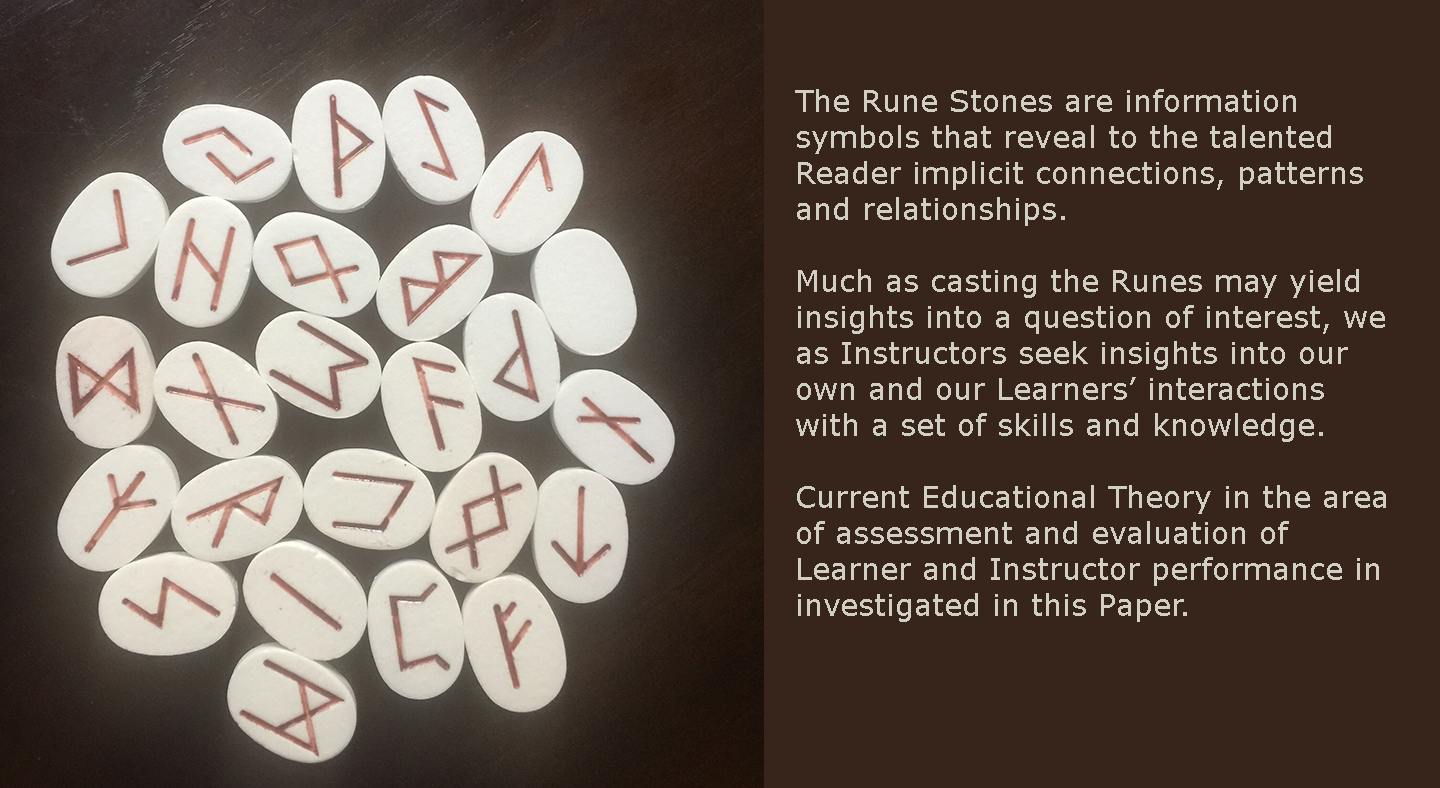
\includegraphics[width=1\textwidth]{images/RuneStones.png}
	\else
    	
\includegraphics{images/cover.jpg}
    \fi
  \end{center}
\newpage
\fi

\begin{chapterpage}{}{p1_foreword:cha}

\begin{myquotation}\large

The absence of data is not the same thing as "No Information"  \newline 
Mr. Spock, Science Officer, First Officer, USS Enterprise

\end{myquotation}
\vspace{2cm}
\begin{myquotation}\large

If you gotta have it explained to you, you ain't never gonna understand it.\newline

Louis Armstrong, American Stage Musician and Performer. Credited with being formative in the development of the Jazz style of music.

\end{myquotation}
\vspace{2cm}
\end{chapterpage}


% surrounding table of contents either with the appropriate style (PDF) or HTML commands (ebook).
\thispagestyle{empty}
\ifx\HCode\undefined 
	% put table of contents on the left side
	\KOMAoptions{open=left}
\else
	\HCode{<nav epub:type="toc">}
\fi

\tableofcontents

\ifx\HCode\undefined
	\KOMAoptions{open=right}
	% finalize page and clear pagestyle to remove header, reset to chapter beginnings on the right side
	\thispagestyle{empty}\pagestyle{empty}\clearpage
\else
	\HCode{</nav>}
\fi
\newpage

% ---------- Main matter
\mainmatter

% reset to normal page numbering (1, 2, 3, ...)
\pagenumbering{arabic}
    
% switch back to basic chapter design
%  Reset the chapter design to a basic one (no box, just underlined chapter title---used for the back and front matter)

\renewcommand*\chapterheadstartvskip{\vspace*{-3\topskip}} 
\renewcommand*\chapterheadendvskip{
  \vskip-.5\baselineskip
  \noindent
  {\color{gray}\rule{\linewidth}{2pt}}
  \par}
\renewcommand*\chapterformat{}
\renewcommand*{\chapterpagestyle}{empty}
% Replace Replace with First Chapter Name
% Replace p1_firstchapter:cha with your chapter title label (no spaces, only lower case letters)
% Replace the text below \end{chapterpage} and insert your own text.

\begin{chapterpage}{ Assessment and Evaluation in Adult Learning}{p1_firstchapter:cha}

\end{chapterpage}
% -------------------- replace or remove text below and paste your own text ------

\section  {Welcome and Introduction}\label{c1_basicformatting:sec}

\begin{itemize}

\item The purpose of this workshop on Assessment and Evaluation in Adult Learning is to enhance your skills as an Instructor in assessing student learning, and to provide the opportunity to experiment with designing evaluation strategies and measures of student learning progress as well as your effectiveness as an Instructor.

\item The evaluation strategies we development will be based on Chapters 3 and 5 of The Art of Evaluation. This textbook is "a practical introduction to learner evaluation in the various contexts of adult education" (Fenwick and Parsons, 2009)

\end{itemize}

\section {Learning Outcomes}

\subsection {Upon completion of this Workshop, the Learner shall be able to describe the operational differences between }

\begin{enumerate}
	\item Diagnostic Evaluations
	\item Formative Evaluations
	\item Summative Evaluations
\end{enumerate}
And be able to identify where in the Learning Content Delivery Cycle each kind of Evaluation should be implemented, what its purpose it, and how the Instructor will utilize the results.

\subsection {Chapter 3: Planning for Evaluation covers the Topics of }

\begin{enumerate}
	\item Why should the Evaluation take place?
	\item What should be evaluated? What do you want the Learners to know?
	\item What do you want to know?
	\item What does the Institution want to know?
	\item What approaches should be used? Here we are factoring in Validity and Reliability.
	\item How much time and resources do you as the Instructor have to do this?
\end{enumerate}

\subsection{Chapter 5 Topics: Choosing an Evaluation Strategy will present the Map of Assessment Methods that are available to us as Instructors:}
The key question here is: What Objective and Subjective strategies should we use to Evaluate Learners' mastery of the Concepts of Chapters 3 and 5? 

How can we best align the methods, instruments and strategies with the learning outcomes?

Are the strategies appropriate for the different types of evaluations? Diagnostic, formative, summative and teaching/training effectiveness.

The Learner shall be able to articulate the differences between Objective and Subjective Evaluations, and categorize the major assessment methods into each bin:
\begin{enumerate}
	\item The Objective Scale evaluators of Multiple Choice, Matching, True/False, and Fill in the Blanks.
    \item The Subjective evaluators of Short Answer, Narrative, and Essay style tests
    \item Student Demonstration of a Skill (Subjective)
    \item Informal student writing: Class Journals, Short Reflection Papers.
\end{enumerate}

\section  {The Toolboxes of Evaluative Methodologies we will be using to assess and evaluate Learning and Instructional Progress:}

\begin{itemize}
\item Include well designed and effective questions
\item Learner Journals
\item Written assignments
\item Performance observation
\item Using Objective Tests
\end{itemize}

\section  {Diagnostic Evaluation:}

Diagnostic evaluation is used to determine student prior knowledge and is generally done at the beginning of a course before theory is presented. 
	Diagnostic evaluation is also a part of the design process done before a course is created. 

For example, data is collected in a "needs assessment" to determine if training is required; and if so, what needs to be taught and what is required of the learner regarding incoming levels of knowledge and experience. 

Diagnostic evaluation of learning occurs in the class/workshop and goes a step further than the design phase of the needs assessment to uncover student expectations of their learning experience.
	Purposes:
		Assess skills, abilities or levels of achievement
		Reveal causes of learning difficulties
		Direct program modification when necessary
	Examples of Assessment for Diagnostic Evaluation:
		Short Essay - The Student Profile (informal)
		Short Essay/Questionnaire - Individual Report Part I in this course (formal)
		Questionnaire/Survey – Needs Assessment sent to participants before a training event or at enrolment (formal)
		Portfolios (formal) (if done before the course begins as in PLAR. See below)
		Verbal & Non-Verbal Q&A, Performance & Observations – Pre-tests, Games, Meet and greet exercise, etc done during the first class or before a new topic is introduced (informal)


Complete the assessment below to determine your prior knowledge before starting the workshop.
Rate items on the scale of Strongly Disagree, Disagree, Agree, and Strongly Agree by placing an ‘X’ in the appropriate box.

\section  {Grading Rubric:}


\section  {References/Citations}
Fenwick, T. and Parsons, J. The Art of Evaluation: A Resource for Educators and Trainers, 2nd Edition. Thompson Educational Publishing, Inc.

\begin{chapterpage}{Peer Review Questions}{p1_secondchapter:cha}

\end{chapterpage}

% -------------------- replace or remove text below and paste your own text ------
\begin{enumerate}
    \item 	Are the methods, instruments and/or strategies aligned with the learning outcomes? Explain.
    \item 	Are the strategies appropriate for the different types of evaluations? Diagnostic, formative, summative and teaching/training effectiveness. Explain.
    \item 	What concerns (if any) do you have with the strategies, methods, content, etc.?
    \item 	Based on what you have learned about creating objective and subjective strategies, what do you think about the objective and subjective strategies created for this evaluation strategy project? What suggestions do you have for improvement?
    \item 	Assess the layout of the evaluation strategies. Are the instructions for the strategies clear and easy to follow? If not, what suggestions do you have for improvement?
    \item 	Do you have any suggestions for different approaches or instruments that can be used for this evaluation strategy project? If so, why? If not, why not?
\end{enumerate}


%%%%%%%%%%%%%%%%%%%%%%%%%%%%%%%%%%%%%
% Read the /ReadMeFirst/ReadMeFirst.tex for an introduction. Check out the accompanying book "Better Books with LaTeX" for a discussion of the template and step-by-step instructions. The template was originally created by Clemens Lode, LODE Publishing (www.lode.de), mail@lode.de, 8/17/2018. Feel free to use this template for your book project!
%%%%%%%%%%%%%%%%%%%%%%%%%%%%%%%%%%%%%


% Command to add some text into the bibliography (between the title and the list of referenced books)
% See https://tex.stackexchange.com/questions/197061/text-between-index-or-bibliography-title-and-content

\bibpreface{Write here the preface of your list of recommended reading titles. Delete this line to have no preface for this section.}

\ifxetex
	\printbibliography
\else
	\newpage
	\bibliographystyle{plainnat}
	\bibliography{bibliography/english}
\fi


\end{document}